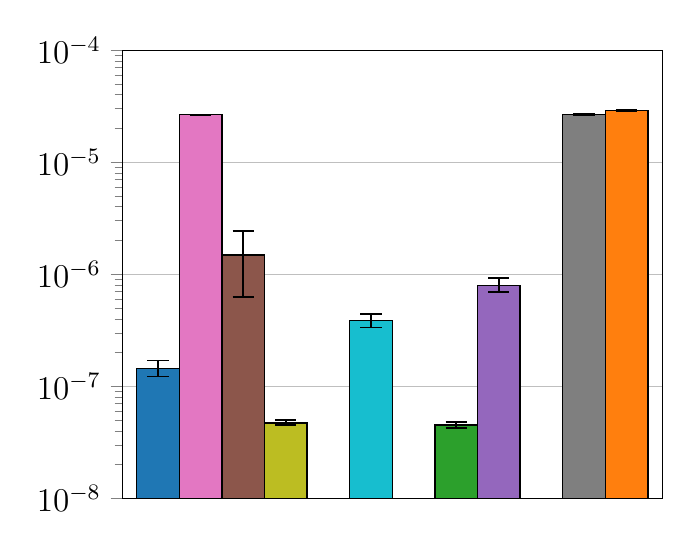
\begin{tikzpicture}
\definecolor{tabblue}{RGB}{31,119,180}
\definecolor{tabgreen}{RGB}{44,160,44}
\definecolor{tabcyan}{RGB}{23,190,207}
\definecolor{tabgray}{RGB}{127,127,127}
\definecolor{taborange}{RGB}{255,127,14}
\definecolor{tabpurple}{RGB}{148,103,189}
\definecolor{tabpink}{RGB}{227,119,194}
\definecolor{tabbrown}{RGB}{140,86,75}
\definecolor{tabolive}{RGB}{188,189,34}

\begin{semilogyaxis}[
  xmin=-0.5, xmax=7.1,
  xtick=\empty,
  ymin=1e-8, ymax=1e-4,
  ymajorgrids,
  ytick pos=left,
  tick align=outside,
  tick label style={font=\large},
]

% Group 1: PEACH/tabblue (0), pstnet/tabpink (0.6), gnn_encoder/tabbrown (1.2), test_opt/tabolive (1.8)
\draw[fill=tabblue,  draw=black, line width=0.5pt] (axis cs:-0.3, 1e-8) rectangle (axis cs:0.3, 1.45e-7);
\draw[fill=tabpink,  draw=black, line width=0.5pt] (axis cs:0.3,  1e-8) rectangle (axis cs:0.9, 2.65e-5);
\draw[fill=tabbrown, draw=black, line width=0.5pt] (axis cs:0.9,  1e-8) rectangle (axis cs:1.5, 1.49e-6);
\draw[fill=tabolive, draw=black, line width=0.5pt] (axis cs:1.5,  1e-8) rectangle (axis cs:2.1, 4.70e-8);

% Group 2: MaNGO/tabcyan (3.0)
\draw[fill=tabcyan,   draw=black, line width=0.5pt] (axis cs:2.7, 1e-8) rectangle (axis cs:3.3, 3.89e-7);

% Group 3: Oracle/tabgreen (4.2), Oracle MGN/tabpurple (4.8)
\draw[fill=tabgreen,  draw=black, line width=0.5pt] (axis cs:3.9, 1e-8) rectangle (axis cs:4.5, 4.52e-8);
\draw[fill=tabpurple, draw=black, line width=0.5pt] (axis cs:4.5, 1e-8) rectangle (axis cs:5.1, 7.92e-7);

% Group 4: No Context/tabgray (6.0), No Context MGN/taborange (6.6)
\draw[fill=tabgray,   draw=black, line width=0.5pt] (axis cs:5.7, 1e-8) rectangle (axis cs:6.3, 2.66e-5);
\draw[fill=taborange, draw=black, line width=0.5pt] (axis cs:6.3, 1e-8) rectangle (axis cs:6.9, 2.90e-5);

% Error bars
% tabblue/PEACH (center 0)
\draw[black, semithick] (axis cs:0,    1.22e-7) -- (axis cs:0,    1.70e-7);
\draw[black, semithick] (axis cs:-0.15,1.22e-7) -- (axis cs:0.15, 1.22e-7);
\draw[black, semithick] (axis cs:-0.15,1.70e-7) -- (axis cs:0.15, 1.70e-7);
% tabpink/pstnet (center 0.6)
\draw[black, semithick] (axis cs:0.6,  2.64e-5) -- (axis cs:0.6,  2.66e-5);
\draw[black, semithick] (axis cs:0.45, 2.64e-5) -- (axis cs:0.75, 2.64e-5);
\draw[black, semithick] (axis cs:0.45, 2.66e-5) -- (axis cs:0.75, 2.66e-5);
% tabbrown/gnn_encoder (center 1.2)
\draw[black, semithick] (axis cs:1.2,  6.23e-7) -- (axis cs:1.2,  2.43e-6);
\draw[black, semithick] (axis cs:1.05, 6.23e-7) -- (axis cs:1.35, 6.23e-7);
\draw[black, semithick] (axis cs:1.05, 2.43e-6) -- (axis cs:1.35, 2.43e-6);
% tabolive/test_opt (center 1.8)
\draw[black, semithick] (axis cs:1.8,  4.49e-8) -- (axis cs:1.8,  5.00e-8);
\draw[black, semithick] (axis cs:1.65, 4.49e-8) -- (axis cs:1.95, 4.49e-8);
\draw[black, semithick] (axis cs:1.65, 5.00e-8) -- (axis cs:1.95, 5.00e-8);
% tabcyan/MaNGO (center 3.0)
\draw[black, semithick] (axis cs:3.0,  3.34e-7) -- (axis cs:3.0,  4.44e-7);
\draw[black, semithick] (axis cs:2.85, 3.34e-7) -- (axis cs:3.15, 3.34e-7);
\draw[black, semithick] (axis cs:2.85, 4.44e-7) -- (axis cs:3.15, 4.44e-7);
% tabgreen/oracle (center 4.2)
\draw[black, semithick] (axis cs:4.2,  4.23e-8) -- (axis cs:4.2,  4.81e-8);
\draw[black, semithick] (axis cs:4.05, 4.23e-8) -- (axis cs:4.35, 4.23e-8);
\draw[black, semithick] (axis cs:4.05, 4.81e-8) -- (axis cs:4.35, 4.81e-8);
% tabpurple/mgn_oracle (center 4.8)
\draw[black, semithick] (axis cs:4.8,  6.98e-7) -- (axis cs:4.8,  9.29e-7);
\draw[black, semithick] (axis cs:4.65, 6.98e-7) -- (axis cs:4.95, 6.98e-7);
\draw[black, semithick] (axis cs:4.65, 9.29e-7) -- (axis cs:4.95, 9.29e-7);
% tabgray/No Context (center 6.0)
\draw[black, semithick] (axis cs:6.0,  2.64e-5) -- (axis cs:6.0,  2.69e-5);
\draw[black, semithick] (axis cs:5.85, 2.64e-5) -- (axis cs:6.15, 2.64e-5);
\draw[black, semithick] (axis cs:5.85, 2.69e-5) -- (axis cs:6.15, 2.69e-5);
% taborange/No Context MGN (center 6.6)
\draw[black, semithick] (axis cs:6.6,  2.85e-5) -- (axis cs:6.6,  2.94e-5);
\draw[black, semithick] (axis cs:6.45, 2.85e-5) -- (axis cs:6.75, 2.85e-5);
\draw[black, semithick] (axis cs:6.45, 2.94e-5) -- (axis cs:6.75, 2.94e-5);

\end{semilogyaxis}
\end{tikzpicture}